% Figures transferred from the working Results; sources are in results-data/.
\newcommand{\diversityfigure}{%
\begin{figure}[htbp]
\centering
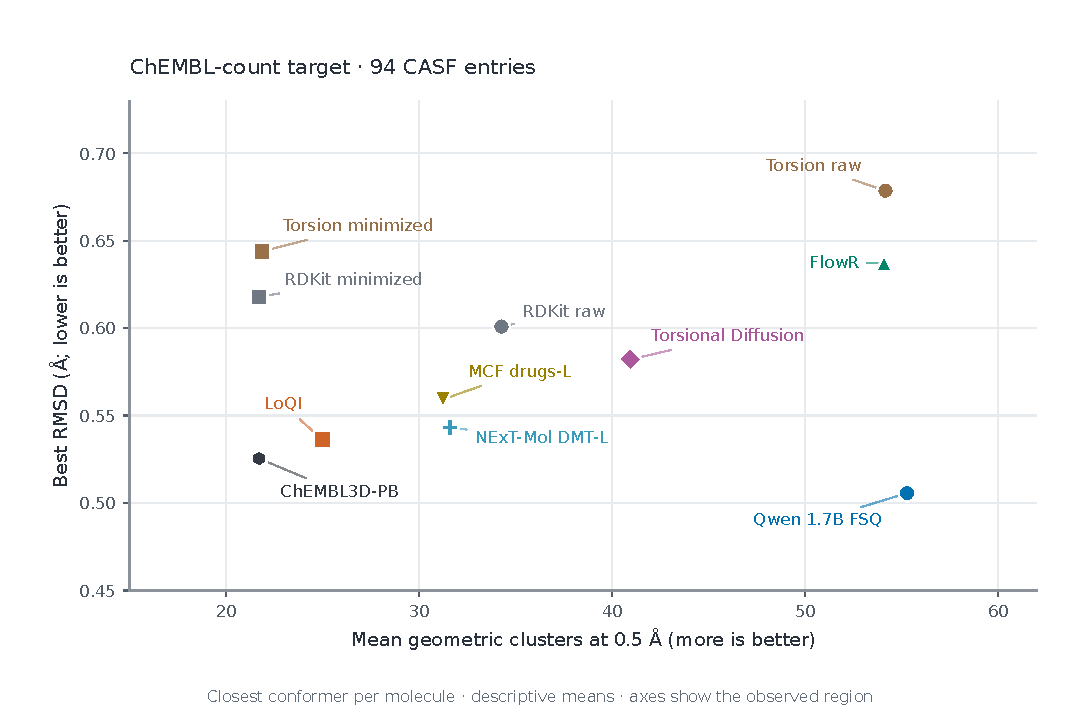
\includegraphics[width=\linewidth]{figures/figure-2-diversity-recovery.pdf}
\caption{Geometric diversity and experimental recovery at the ChEMBL-count target. Each point represents one evaluated pipeline or the stored ChEMBL3D-PB ensemble. Clustering uses a 1.0 \AA{} radius, whereas recovery requires at least one retained conformer at RMSD $\leq$ 0.75 \AA{}. Cluster counts are averaged over defined measurements; recovery uses all 94 entries, including failures. Retained ensemble sizes differ despite matched candidate targets. These are descriptive method summaries, not a causal analysis of diversity.}
\label{fig:diversity-recovery}
\end{figure}}

\newcommand{\recoveryfigure}{%
\begin{figure}[htbp]
\centering
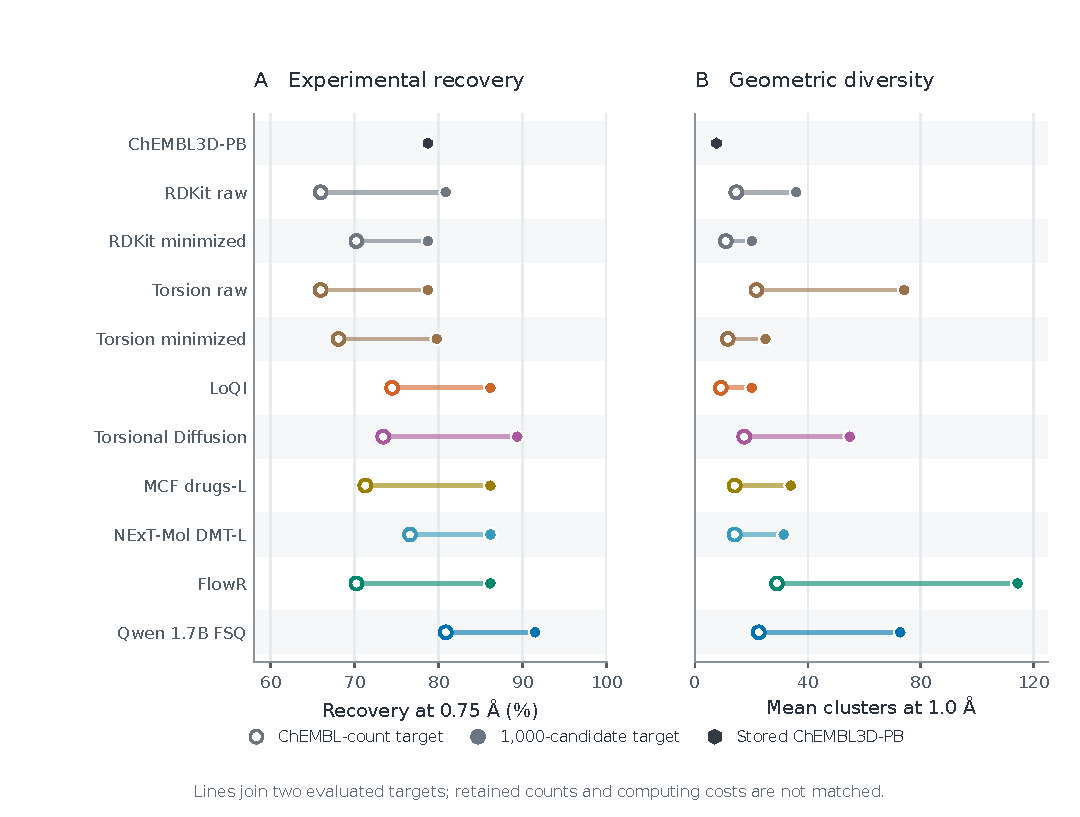
\includegraphics[width=\linewidth]{figures/figure-3-sampling-budget.pdf}
\caption{Recovery and diversity at the two candidate targets. Open circles denote the ChEMBL-count target and filled circles the 1,000-candidate target. Each row follows the same method between the two targets. The stored ChEMBL3D-PB ensemble is shown once as a hexagon. Recovery uses all 94 CASF entries; cluster means use defined measurements. Lines connect observed endpoints and do not represent random-subsampling curves or intermediate measurements. Targets precede PoseBusters filtering; retained counts are given in Table~\ref{tab:recovery}.}
\label{fig:recovery}
\end{figure}}

\newcommand{\sizefigure}{%
\begin{figure}[htbp]
\centering
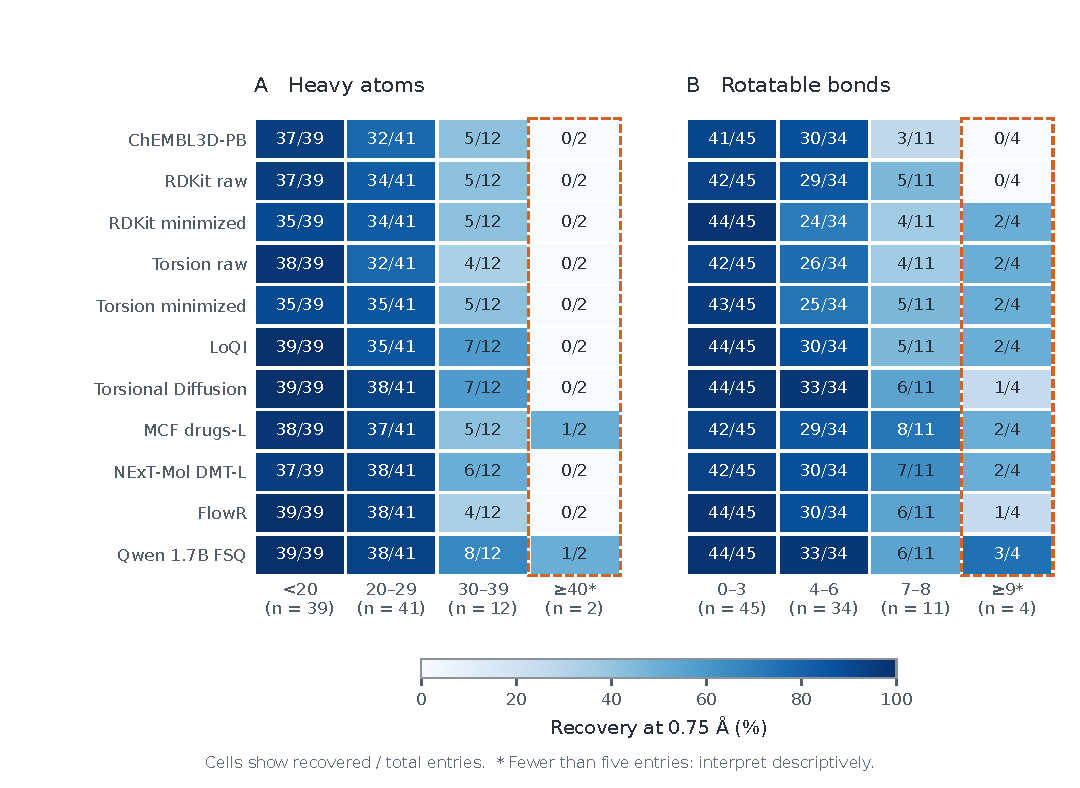
\includegraphics[width=\linewidth]{figures/figure-4-size-flexibility.pdf}
\caption{Recovery by molecular size and flexibility. Generated methods use the 1,000-candidate target; ChEMBL3D-PB uses its stored ensemble. Every cell gives recovered/total CASF entries, with the color indicating the corresponding percentage. Dashed outlines mark groups with fewer than five entries. Heavy-atom and rotatable-bond groups are analyzed separately and do not isolate independent effects of size and flexibility. Sparse groups cannot establish stable method rankings.}
\label{fig:size}
\end{figure}}

\newcommand{\drugfigure}{%
\begin{figure}[htbp]
\centering
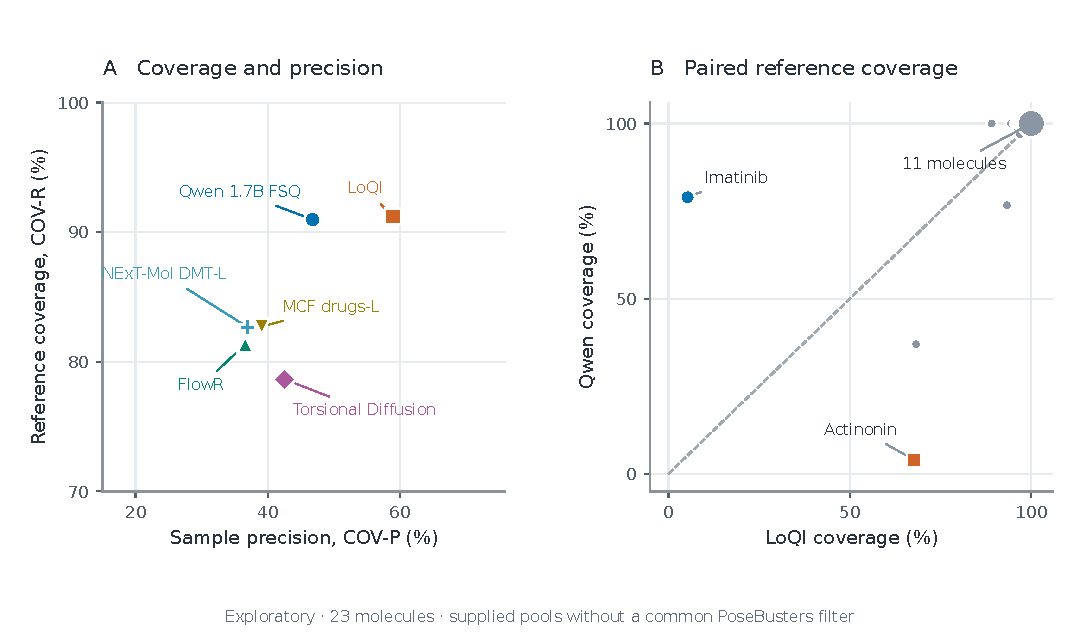
\includegraphics[width=\linewidth]{figures/figure-5-multiple-references.pdf}
\caption{Coverage of multiple bound references and precision relative to those observations. (A) Molecule-averaged COV-R and COV-P for six learned generators, using the existing strict RMSD $<$ 0.75 \AA{} criterion. Axes are restricted to the observed range for readability. (B) Paired reference coverage for Qwen and LoQI across all 23 molecules; the diagonal denotes equal coverage. Coincident points are grouped and labeled, including 11 molecules with complete coverage by both methods. Imatinib and actinonin are the examples retained from the earlier draft. These are descriptive supplied-pool results with differing RMSD-failure conventions, not a comparison after common validity filtering. No uncertainty intervals are shown; paired uncertainty is documented in the archived findings.}
\label{fig:druglike}
\end{figure}}
